% To add an image or include a .tex file you need to add
% \CWD
% to the relative (to the main document) path.
%
% Example:
% \begin{figure}
%   \centering
%   \includegraphics{\CWD/images/example.pdf}
% \end{figure}

A Avenida do Contorno é uma avenida circular de Belo Horizonte. Durante sua construção, foram instaladas vários estabelecimentos ao longo dela, como várias drogarias (Araújo), várias pastelarias (Rei do Pastel), etc. Por motivos logísticos, todo par de estabelecimentos do mesmo tipo deve ser conectado \textbf{diretamente} por uma rua (que pode passar por dentro ou por fora da Contorno).

Porém, para que a Contorno continue sendo a avenida principal, não podem existir esquinas em outros lugares da cidade (cruzamento de ruas). Além disso, não irão existir túneis ou viadutos na cidade.

Dados os tipos de estabelecimentos que existem em ordem ao longo da Contorno, sua tarefa é determinar se é possível construir as ruas conectando todo par de estabelecimentos de mesmo tipo, sem criar esquinas (cruzamentos de ruas) extras.

\begin{figure}[H]
  \centering
  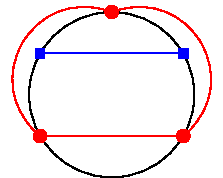
\includegraphics[scale=1.5]{\CWD/img/image.pdf}
  \caption{Possível configuração para o primeiro exemplo.}
\end{figure}

%
% For input, use one of the following
%
\inputdesc{A primeira linha contém um inteiro $1 \leq N \leq 10^3$. A segunda linha contém $N$ inteiros $1 \leq c_i \leq N$, em que $c_i$ representa o tipo do $i$-ésimo estabelecimento em ordem na Contorno.}

%
% For output, use one of the following
%

\outputdesc{Imprima {\tt S} caso seja posssível construir as estradas, e {\tt N} caso contrário.}

\section*{Restrições}

\begin{itemize}
\item $1 \leq N \leq 10^3$.
\end{itemize}

%\sampleio will look for files named sample-n.in and sample-n.sol (where n is 1, 2, 3...)
%in the documents directory and include them as samples.

\sampleio
